% \section{Information Theory}
Information theory provides us the tools to study the information processing capabilities of different systems. These systems include computers, artificial intelligence and also the brain. The story of Information Theory begins with Shannon who provided the tools to estimate information \cite{shin1949mathematical}. The most fundamental aspect of information theory is the concept of the 'bit'. 

As a standard, information theory deals with 'bits'. One bit of information represents a choice between two equally probable options. A perfectly balanced coin toss contains one bit of information. It has 50\% chance of landing on head and 50\% chance of landing on tails. A bit is a measure of information and a measure of uncertainty. Thus uncertainty and information are tightly intertwined. If we are completely certain about a certain event, there is no information to be gained. 

This chapter will cover the most important aspects of information theory. First and formost, this means discussing entropy. Once we have an understanding of entropy, extensions can be discussed. These include joint entropy and conditional entropy. With these tools, we can go into the area of mutual information, which plays an important role in this thesis. Another important aspect is the generalisation into multivariate systems and dealing with continuous (as opposed to discrete) systems. Finally, some explanation is provided of coding theory and cybernetics.

\section{Entropy}

The next step is entropy. There are different kinds of entropy, such as thermodynamic entropy. Here, we are talking about information entropy. Information entropy is the average uncertainty associated with a random variable. In other words, information entropy is the average rate of information from a random or stochastic variable. 

In order to calculate the entropy, we require some discrete random variable X, with ${x_1 ... x_n}$ the different values from X. $P(x)$ is the probability mass function. The entropy $H(X)$ can be calculated as:

\begin{equation}
H(X) = -\sum_{i=1}^{n}P(x_i)log_2(P(x_i))
\end{equation}

Interesting to note is that $log_2(P(x_i))$ is the information about value $x_i$. This formula can be extended into the conditional entropy of two events $X$ and $Y$. The entropy $H(X|Y)$ is the entropy of random variable X given that the outcome of Y is known.

\begin{equation}
H(X|Y) = \sum_{i,j}P(x_i, y_j)log_2(\frac{P(y_j)}{P(x_i, y_j)}) = -\sum_{i,j}P(x_i, y_j)log_2(\frac{P(x_i, y_j)}{P(y_j)})
\end{equation}

If random variables X and Y are independent of eachother, then $H(X|Y) = H(X)$. If the variables are completely independent, knowing anything about Y, will not change anything we know about X. Similarly, if $H(X|Y) = 0$, then X is completely determined by Y. 

The rule of Bayes is also applicable to conditional entropy:

\begin{equation}
H(X|Y) = H(Y|X) + H(Y) - H(X)
\end{equation}

\section{Joint Entropy}

$H(X)$ and $H(X|Y)$ are basic notions of information measures. Figure~\ref{entropy} visualises the notion of entropy. This figure also contains two information measures that are not yet described, $I(X,Y)$ and $H(X,Y)$. Respectively, they are the mutual information and the joint entropy.

\begin{figure}[!htb]
\caption{Venn diagram for information measures.}
\label{entropy}
    \centering
    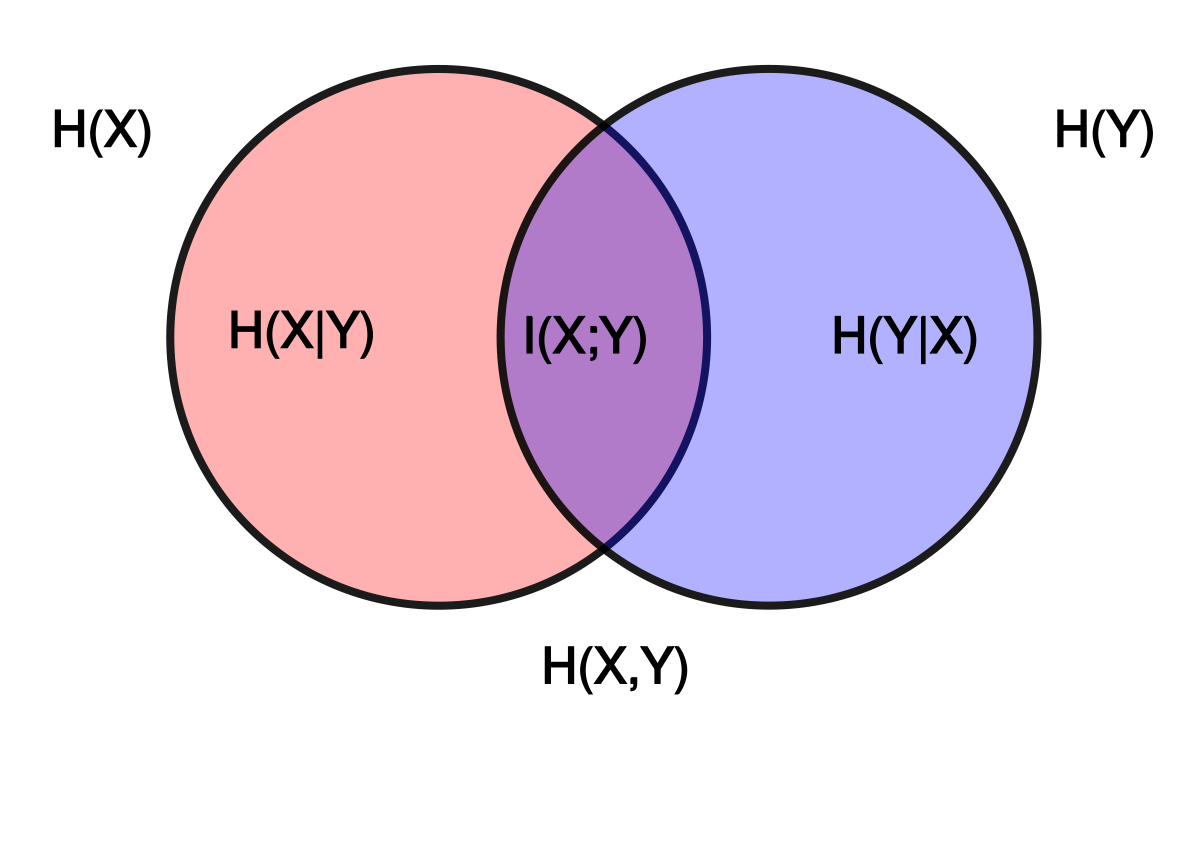
\includegraphics[width=0.8\textwidth]{fig/entropy}
\end{figure}

In the figure, $H(X,Y)$ is the complete information content of X and Y. Using the following equation, we can calculate $H(X,Y)$:

\begin{equation}
H(X,Y) = -\sum_{i=1}^{n}\sum_{j=1}^{m}P(x_i, y_j)log_2(P(x_i, y_j))
\end{equation}

Using figure~\ref{entropy}, we can see some interesting relations. $H(X,Y)$ is related to $H(X|Y)$ and $H(X)$:
\begin{equation}\label{joint}
H(X,Y) = H(X|Y) + H(Y)
\end{equation}

This can be validated:
\begin{align*}
H(X,Y) &= -\sum_{i=1}^{n}\sum_{j=1}^{m}P(x_i, y_j)log_2(P(x_i, y_j))\\
&= -\sum_{i=1}^{n}\sum_{j=1}^{m}P(x_i, y_j)log_2(P(y_i)P(x_i | y_j))\\
&= -\sum_{i=1}^{n}\sum_{j=1}^{m}P(x_i, y_j)log_2(P(y_i))-\sum_{i=1}^{n}\sum_{j=1}^{m}P(x_i, y_j)log_2(P(x_i | y_j))\\
&= -\sum_{j=1}^{m}P(y_j)log_2(P(y_i))-\sum_{i=1}^{n}\sum_{j=1}^{m}P(x_i, y_j)log_2(P(x_i | y_j))\\
&= H(Y) + H(X|Y)
\end{align*}

This relation is useful for the actual implementation of information theoretical algorithms. An important note about entropy, conditional entropy and joint entropy is that they are non-negative. It would not make sense for an random variable to have a negative information content. Joint entropy is also always greater or equal to individual entropy and joint entropy is smaller or equal to the sum of individual entropies.

\begin{equation}
H(X) \ge 0
\end{equation}

\begin{equation}
H(X|Y) \ge 0
\end{equation}

\begin{equation}
H(X,Y) \ge 0
\end{equation}

\begin{equation}
H(X,Y) \ge H(X)
\end{equation}

\begin{equation}
H(X,Y) \le H(X) + H(Y) 
\end{equation}

\section{Mutual Information}
Mutual information is the amount of information that is common between two variables. Figure~\ref{entropy} shows the mutual information as the intersection between $H(X)$ and $H(Y)$. The figure also shows how mutual information can be computed. The individual entropies are summed and the joint entropy is subtracted. Another equal interpretation of mutual information is that mutual information measures the reduction in uncertainty or information when we observe one of the variables.

\begin{equation}
I(X,Y) = H(X) + H(Y) - H(X,Y)
\end{equation}

\begin{equation}
I(X,Y) = H(X) - H(X|Y)
\end{equation}

Mutual information can also be calculated using the probability mass functions directly. In this case we get:

\begin{equation}
I(X,Y) = \sum_{i=1}^{n}\sum_{j=1}^{m}P(x_i, y_j)log_2(\frac{P(x_i, y_j)}{P(x_i)P(y_j)})
\end{equation}
    
While mutual information does show whether there is a relationship or correlation between two variables, it does not give information about the "shape" of the relationship. Making the analogy with figure~\ref{entropy}, mutual information shows how much overlap there is, but it does not explain anything else. Mutual information makes no assumptions of what the distribution of the variables X and Y is like. 

Mutual information, like entropy, is non-negative. Additionally, just like there is conditional entropy, there is also conditional mutual information. Conditional mutual information indicates the mutual information given another variable is given:

\begin{equation}
I(X,Y|Z) = \sum_{k=1}^{o}\sum_{i=1}^{n}\sum_{j=1}^{m}P(x_i, y_j, z_k)log_2(\frac{P(x_i, y_j z_k)P(z_k)}{P(x_i, z_k)P(y_j z_k)})
\end{equation}

\section{Multi-Variate Information Theory}
In the previous sections, information theory has been observed through a bivariate lens. These methods can be generalised to multivariate variations. When comparing different brain regions, we do not want to restrict ourselves to a bivariate case.

Joint entropy can be easily extended to a multivariate case. In the bivariate case, the joint probability mass function was used and a summation over both random variables was done. The multivariate case simply generalises this equation:

\begin{equation}
H(X_1, ..., X_n) = -\sum_{x_1}...\sum_{x_n}P(x_1,...,x_n)log_2(P(x_1,...,x_n))
\end{equation}

Equation~\ref{joint} can also be extended into a multivariate case. In this case, we get:

\begin{equation}
H(X_1, ..., X_n) = -\sum_{k=1}^{n}H(X_k|X_{k-1},...,X_1)
\end{equation}

The multivariate case of conditional entropy becomes:

\begin{equation}
H(Y | X_1, ..., X_n) = H(Y, X_1, ..., X_n) - H(X_1, ..., X_n)
\end{equation}

Having extended the different forms of entropy into a multivariate case, we can make a multivariate method for mutual information. The multivariate mutual information becomes a recursive function:

\todo{add mutual information + conditional}

\section{Continuous Data}

\todo{explain that we have continuous data, not discrete}

\section{Coding Theory}

\section{Cybernetics}